\section{Optimized Grid Model}
\setlength{\parindent}{10ex}
%Purpose of this section is to identify the optimized grid structure.
%I need to check with Hoque to identify what I should and shouldnt include
%I need to consider rewording this and restructuring to manage the correctness for example etc.
Further analysis of figure \ref{fig:rfc_report} shows that models are sensitive to potentially local characteristics.
In an attempt to test this notion and increase the accuracy of these models a novel model selection method was employed.
The objective being to identify if a model will predict more accurately based on geospatial location.
The hypothesis being that decision boundaries across different models will respond to features based on location.

The Grid Optimized Model Injector Classifier was created to test this theory.
This model is built upon the idea that there is not a optimal single model for predicting all of the worlds bathymetry.
It leverages several different models to predict bathymetry in a area by recording the best preforming models across a grid of the world.
This allows the model to use the optimal model for predicting bathymetry.

%Give the background for the idea in this section!
\subsection{Analysis of Global Model Optimization}
Testing this hypothesis was performed by splitting the world into coverages.
Each coverage represented a exclusive area of the Earth's ocean.
A set of models were trained on each coverage and their prediction accuracy's were compared.
The most accurate model was then saved for each coverage and stored in a map.
The results of this script are displayed in figure \ref{fig:coveragegrid}.

\begin{figure}[htp]
    \centering
    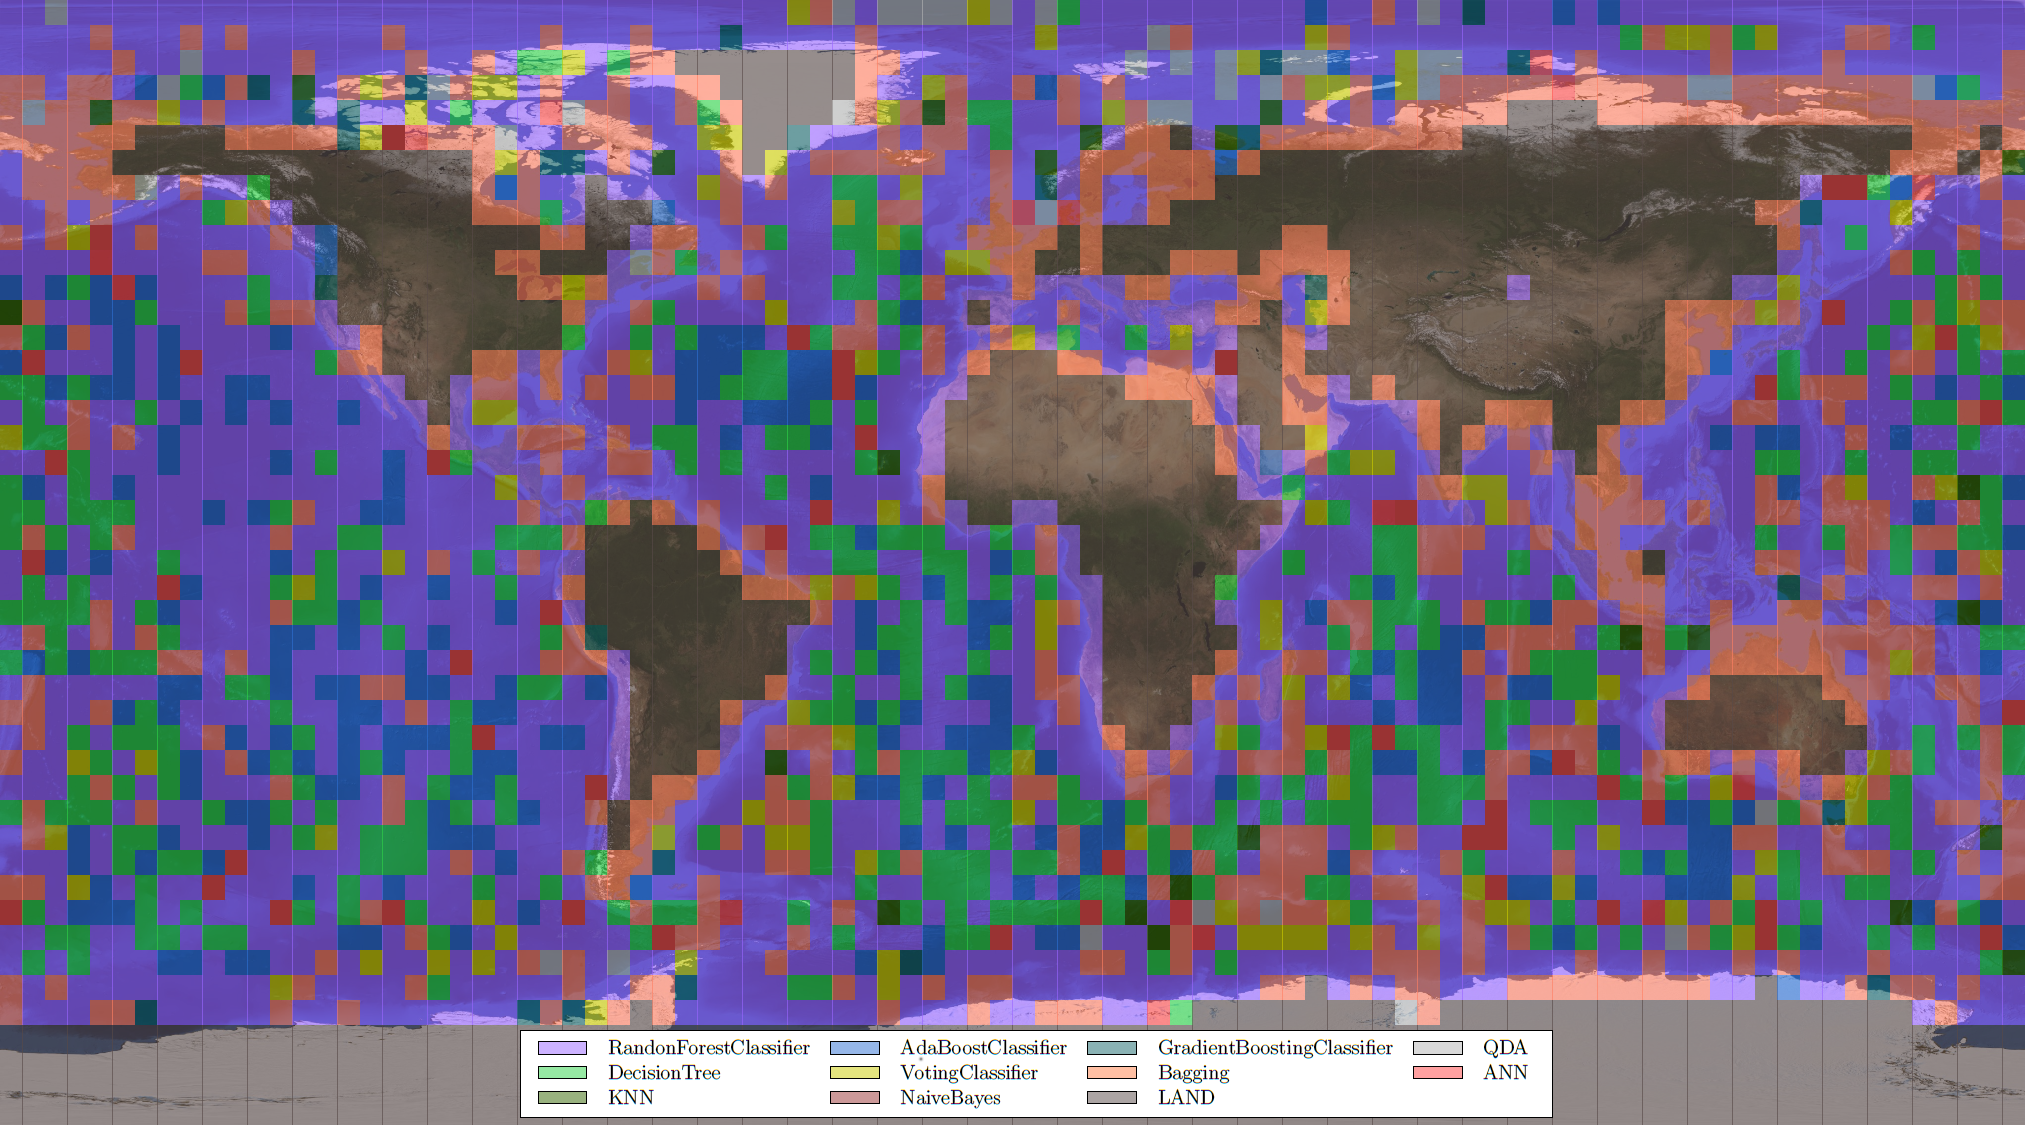
\includegraphics[width=\textwidth]{optgriddraft.png}
    \caption{Graphic Showing the World Coverages and Successful Models}
    \label{fig:coveragegrid}
\end{figure}

\par
Clearly, figure \ref{fig:coveragegrid} provides evidence that model decision boundaries are sensitive to the features based on location.
Leading to the conclusion that there is not a single best fit model for predicting global bathymetry.
Analysis of figure \ref{fig:coveragegrid} shows interesting consistencies that raise questions about the underlying features.
For example, the decision tree classifier preformed poorly as configured in the classification section when used for global predictions.
When predicting near fault lines it preformed the best out of other models.
Bagging seemed to dominate on coast lines while \ac{RFC} performed best in open waters.

%In this section I am defining what the Grid optimization is and why it matters.
%There may be a better name for this?? Who knows really...
\subsection{Grid Optimizing}
The results of the experiment were then used for model selection.
Using the successful model for each coverage as a \textit{optimum} selection.
A trivial geospatial query is used to query the best model by location.
This selection is implemented in a novel model I call the \textit{Grid Optimized Model Injector Classifier}.
This name is chosen because the result model acquired from the spatial query is injected for classification.

%This is where I define what happens after the appropriate coverages have been found.
\par
In theory, this injection will allow each model to perform to its optimum.
Each coverage highlights distinct characteristics that will produce a better decision boundary.
These coverages are simple partitions of the world, but could be extended in future work to optimize the selection.
% Reconsider this sentence....


\subsection{Results and Discussion}
%The world wide ETOPO bathymetry dataset \cite{national1988etopo} at two minute resolution is used for valadation and metrics.
%This dataset is treated as the ground truth for all predictions.
%During the experiment, a one third holdout was used for validation in some cases.
%For finding the optimum model for a coverage a 10 fold cross validation was utilized.

%Include metrics information here.... possibly graphs and a list of scores? I dont really know.

%I dont like how I worded this whole section...
%The idea here is that I want to say "Hey, these people did this research and found the their regression model preforms poorly for predicting seamounts espicially after 500m.
%I clearly noticed a similar trend, but saw better preformance from some models than others. 
%This research is to identify those coverages and then use those results to build a super classifier.
%These metrics are important for identifying where the models preform well. 
\par
The Grid Optimized Model Injector improved the accuracy of predictions by \~{}5\%.
These results are displayed in table \ref{table:GRID_OPT_RESULTS}.
Obviously, the model selection and subsequent injection improved the results of this classifier.
Creating a ensemble of many models and selecting them on demand.
This could be caused by geophysical characteristics that benefit one classifier.
For example, in figure \ref{fig:coveragegrid} the Decision Tree classifier preformed best along what appears to be fault lines.
It is possible that the characteristics related to being in proximity to a fault line benefited the models decision boundary. 

\begin{table}[htp]
    \centering
    \begin{tabular}{|c c c|}
        \hline
        \textbf{Model} & \textbf{Average F1 Score} & \textbf{Mean Balanced Accuracy} \\
		\hline
		Grid Optimized Model Injector & 0.83 & 0.862 \\
		\hline
    \end{tabular}
    \label{table:GRID_OPT_RESULTS}
    \caption{Grid Optimized Model Injector Results}
\end{table}

\par
In any event, there is evidence to support geophysical location drives the factors that help predict bathymetry.
Things to optimize may include investigating the appropriate feature sets, coverage boundaries, depth boundaries, parameters, and metrics based on geophysical location.
For example, volcanic activity creates new land.
This activity has a causal relationship to bathymetry, but volcanic activity at a specific point may not affect the bathymetry at a potential antipodal point.
Another example being that the coverage boundaries are potentially a naive selection choice.
It is possible that choosing models by performance across depth boundaries proves to be a better selector.
%Extending off the research preformed in \cite{jena2012prediction} these metrics allow the selection of the best preforming model.

%Maybe here I can have a table show casing the preformance of models or possibly statistics about the coverages??
%It will be intersting to see what has preformed better across the globe
%Also is intersting to see which models have preformed best overall.
